\documentclass{standalone}
\usepackage{tikz,,calc}
\usetikzlibrary{intersections, calc}
\renewcommand{\familydefault}{\sfdefault}


\tikzset{
    partial ellipse/.style args={#1:#2:#3}{
        insert path={+ (#1:#3) arc (#1:#2:#3)}
    }
}

\begin{document}
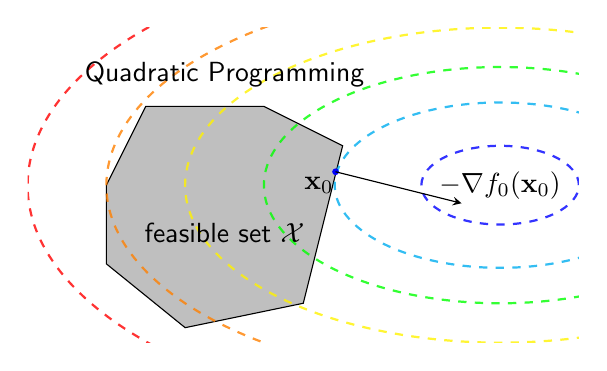
\begin{tikzpicture}[>=stealth]
  \clip (-1, -1) rectangle (6, 3);
  % \begin{scope}[xshift = 6cm]
  \draw [fill = gray!50] (0, 0) -- (1, -.81) -- (2.5, -.5) -- (3, 1.5) -- (2, 2) -- (.5, 2) -- (0, 1) -- cycle;
  
  \def\k{5.25}
  \def\ax{2.65}
  \def\bx{3.4}
  \def\ay{\d*(\ax - 3) + 1}

  \def\r{2}
  \draw[thick, dashed, opacity = .8, blue] (5,1) [partial ellipse=0:360:1cm and .5cm];
  \def\r{2.1}
  \draw[thick, dashed, opacity = .8, cyan] (5,1) [partial ellipse=30:330:\r cm and .5*\r cm];
  \draw[thick, dashed, opacity = .8, green] (5,1) [partial ellipse=30:330:3cm and 1.5cm];
  \draw[thick, dashed, opacity = .8, yellow] (5,1) [partial ellipse=30:330:4cm and 2cm];
  \draw[thick, dashed, opacity = .8, orange] (5,1) [partial ellipse=30:330:5cm and 2.5cm];
  \draw[thick, dashed, opacity = .8, red] (5,1) [partial ellipse=30:330:6cm and 3cm];

  \draw [fill = blue, draw = blue] (2.91, 1.17 ) circle (1pt);
  \def\a{.4}
  \draw [->](2.91, 1.17) -- (2.91 + 4*\a, 1.17 - \a);
  \node at (5, 1) {$-\nabla f_0 (\mathbf{x}_0)$};
  % \draw [fill = red, draw = red] (0, 1 ) circle (1pt);

  \node at (1.5, 0.4) {feasible set $\mathcal{X}$};
  \node at (1.5, 2.4) {Quadratic Programming};
  \node at (2.7, 1) {$\mathbf{x}_0$};
  % \node at (.3, 1) {$\mathbf{x}_1$};
  % \node at (4.3, 1) {$-\mathbf{c}$};

  % \coordinate (P) at ($(0, 0) + (30:3cm and 2cm)$);

  % \draw[thick, red, -latex] ($(0, 0) + (30:3cm and 2cm)$(P) arc
  % (30:150:3cm and 2cm);


  % \draw (-1, .5) -- (3, -1.5);
  % \draw (1.5, -2) -- (3.5, 2);
  % \draw (-.5, .75) -- (3, 2.5);
  % \draw (0, -1) -- (0, 2);
  % \draw (3.5, .5) -- (1.5, 2.5);

  % \end{scope}
\end{tikzpicture}
\end{document} 